% !TeX spellcheck = pl_PL
%%%%%%%%%%%%%%%%%%%%%%%%%%%%%%%%%%%%%%%%%%%
%                                        %
% Szablon pracy dyplomowej inzynierskiej %
% zgodny  z aktualnymi  przepisami  SZJK %
%                                        %
%%%%%%%%%%%%%%%%%%%%%%%%%%%%%%%%%%%%%%%%%%
%                                        %
%  (c) Krzysztof Simiński, 2018-2023     %
%                                        %
%%%%%%%%%%%%%%%%%%%%%%%%%%%%%%%%%%%%%%%%%%
%                                        %
% Najnowsza wersja szablonów jest        %
% podstępna pod adresem                  %
% github.com/ksiminski/polsl-aei-theses  %
%                                        %
%%%%%%%%%%%%%%%%%%%%%%%%%%%%%%%%%%%%%%%%%%
%
%
% Projekt LaTeXowy zapewnia odpowiednie formatowanie pracy,
% zgodnie z wymaganiami Systemu zapewniania jakości kształcenia.
% Proszę nie zmieniać ustawień formatowania (np. fontu,
% marginesów, wytłuszczeń, kursywy itd. ).
%
% Projekt można kompilować na kilka sposobów.
%
% 1. kompilacja pdfLaTeX
%
% pdflatex main
% bibtex   main
% pdflatex main
% pdflatex main
%
%
% 2. kompilacja XeLaTeX
%
% Kompilatacja przy użyciu XeLaTeXa różni się tym, że na stronie
% tytułowej używany jest font Calibri. Wymaga to jego uprzedniego
% zainstalowania.
%
% xelatex main
% bibtex  main
% xelatex main
% xelatex main
%
%
%%%%%%%%%%%%%%%%%%%%%%%%%%%%%%%%%%%%%%%%%%%%%%%%%%%%%
% W przypadku pytań, uwag, proszę pisać na adres:   %
%      krzysztof.siminski(małpa)polsl.pl            %
%%%%%%%%%%%%%%%%%%%%%%%%%%%%%%%%%%%%%%%%%%%%%%%%%%%%%
%
% Chcemy ulepszać szablony LaTeXowe prac dyplomowych.
% Wypełniając ankietę spod poniższego adresu pomogą
% Państwo nam to zrobić. Ankieta jest całkowicie
% anonimowa. Dziękujemy!


% https://docs.google.com/forms/d/e/1FAIpQLScyllVxNKzKFHfILDfdbwC-jvT8YL0RSTFs-s27UGw9CKn-fQ/viewform?usp=sf_link
%
%%%%%%%%%%%%%%%%%%%%%%%%%%%%%%%%%%%%%%%%%%%%%%%%%%%%%%%%%%%%%%%%%%%%%%%%%

%%%%%%%%%%%%%%%%%%%%%%%%%%%%%%%%%%%%%%%%%%%%%%%
%                                             %
% PERSONALIZACJA PRACY – DANE PRACY           %
%                                             %
%%%%%%%%%%%%%%%%%%%%%%%%%%%%%%%%%%%%%%%%%%%%%%%

% Proszę wpisać swoje dane w poniższych definicjach.

% TODO
% dane autora
\newcommand{\FirstNameAuthor}{Maciej}
\newcommand{\SurnameAuthor}{Waleryn}
\newcommand{\IdAuthor}{296441}   % numer albumu  (bez $\langle$ i $\rangle$)

% drugi autor:
%\newcommand{\FirstNameCoauthor}{Imię}   % Jeżeli jest drugi autor, to tutaj należy podać imię.
%\newcommand{\SurnameCoauthor}{Nazwisko} % Jeżeli jest drugi autor, to tutaj należy podać nazwisko.
%\newcommand{\IdCoauthor}{$\langle$wpisać właściwy$\rangle$}  % numer albumu drugiego autora (bez $\langle$ i $\rangle$)
% Gdy nie ma drugiego autora, należy zostawić poniższe definicje puste, jak poniżej. Gdy jest drugi autor, należy zakomentować te linie.
\newcommand{\FirstNameCoauthor}{} % Jeżeli praca ma tylko jednego autora, to dane drugiego autora zostają puste.
\newcommand{\SurnameCoauthor}{}   % Jeżeli praca ma tylko jednego autora, to dane drugiego autora zostają puste.
\newcommand{\IdCoauthor}{}  % Jeżeli praca ma tylko jednego autora, to dane drugiego autora zostają puste.
%%%%%%%%%%

\newcommand{\Supervisor}{dr hab. inż. Krzysztof Simiński}     % dane promotora (bez $\langle$ i $\rangle$)
\newcommand{\Title}{Język programowania dla mikrokontrolerów AVR}           % tytuł pracy po polsku
\newcommand{\TitleAlt}{Programming language for AVR microcontrollers}                     % thesis title in English
\newcommand{\Program}{Informatyka}            % kierunek studiów  (bez $\langle$ i $\rangle$)
\newcommand{\Specialisation}{Grafika komputerowa}     % specjalność  (bez $\langle$ i $\rangle$)
\newcommand{\Departament}{Algorytmiki i Oprogramowania}        % katedra promotora  (bez $\langle$ i $\rangle$)

% Jeżeli został wyznaczony promotor pomocniczy lub opiekun, proszę go/ją wpisać ...
\newcommand{\Consultant}{$\langle$stopień naukowy imię i nazwisko$\rangle$} % dane promotora pomocniczego, opiekuna (bez $\langle$ i $\rangle$)
% ... w przeciwnym razie proszę zostawić puste miejsce jak poniżej:
%\newcommand{\Consultant}{} % brak promotowa pomocniczego / opiekuna

% koniec fragmentu do modyfikacji
%%%%%%%%%%%%%%%%%%%%%%%%%%%%%%%%%%%%%%%%%%


%%%%%%%%%%%%%%%%%%%%%%%%%%%%%%%%%%%%%%%%%%%%%%%
%                                             %
% KONIEC PERSONALIZACJI PRACY                 %
%                                             %
%%%%%%%%%%%%%%%%%%%%%%%%%%%%%%%%%%%%%%%%%%%%%%%

%%%%%%%%%%%%%%%%%%%%%%%%%%%%%%%%%%%%%%%%


%%%%%%%%%%%%%%%%%%%%%%%%%%%%%%%%%%%%%%%%%%%%%%%
%                                             %
% PROSZĘ NIE MODYFIKOWAĆ PONIŻSZYCH USTAWIEŃ! %
%                                             %
%%%%%%%%%%%%%%%%%%%%%%%%%%%%%%%%%%%%%%%%%%%%%%%



\documentclass[a4paper,twoside,12pt]{book}
\usepackage[utf8]{inputenc}                                      
\usepackage[T1]{fontenc}  
\usepackage{amsmath,amsfonts,amssymb,amsthm}
\usepackage[british,polish]{babel} 
\usepackage{indentfirst}
\usepackage{xurl}
\usepackage{xstring}
\usepackage{ifthen}



\usepackage{ifxetex}

\ifxetex
	\usepackage{fontspec}
	\defaultfontfeatures{Mapping=tex—text} % to support TeX conventions like ``——-''
	\usepackage{xunicode} % Unicode support for LaTeX character names (accents, European chars, etc)
	\usepackage{xltxtra} % Extra customizations for XeLaTeX
\else
	\usepackage{lmodern}
\fi



\usepackage[margin=2.5cm]{geometry}
\usepackage{graphicx} 
\usepackage{hyperref}
\usepackage{booktabs}
\usepackage{tikz}
\usepackage{pgfplots}
\usepackage{mathtools}
\usepackage{geometry}
\usepackage{subcaption}   % subfigures
\usepackage[page]{appendix} % toc,
\renewcommand{\appendixtocname}{Dodatki}
\renewcommand{\appendixpagename}{Dodatki}
\renewcommand{\appendixname}{Dodatek}

\usepackage{csquotes}
\usepackage[natbib=true,backend=bibtex,maxbibnames=99]{biblatex}  % kompilacja bibliografii BibTeXem
%\usepackage[natbib=true,backend=biber,maxbibnames=99]{biblatex}  % kompilacja bibliografii Biberem
\bibliography{biblio/biblio}

\usepackage{ifmtarg}   % empty commands  

\usepackage{setspace}
\onehalfspacing


\frenchspacing



%%%% TODO LIST GENERATOR %%%%%%%%%

\usepackage{color}
\definecolor{brickred}      {cmyk}{0   , 0.89, 0.94, 0.28}

\makeatletter \newcommand \kslistofremarks{\section*{Uwagi} \@starttoc{rks}}
  \newcommand\l@uwagas[2]
    {\par\noindent \textbf{#2:} %\parbox{10cm}
{#1}\par} \makeatother


\newcommand{\ksremark}[1]{%
{%\marginpar{\textdbend}
{\color{brickred}{[#1]}}}%
\addcontentsline{rks}{uwagas}{\protect{#1}}%
}

\newcommand{\comma}{\ksremark{przecinek}}
\newcommand{\nocomma}{\ksremark{bez przecinka}}
\newcommand{\styl}{\ksremark{styl}}
\newcommand{\ortografia}{\ksremark{ortografia}}
\newcommand{\fleksja}{\ksremark{fleksja}}
\newcommand{\pauza}{\ksremark{pauza `--', nie dywiz `-'}}
\newcommand{\kolokwializm}{\ksremark{kolokwializm}}
\newcommand{\cudzyslowy}{\ksremark{,,polskie cudzysłowy''}}
\newcommand{\cytowanie}{\ksremark{cytowanie}}

%%%%%%%%%%%%%% END OF TODO LIST GENERATOR %%%%%%%%%%%

\newcommand{\printCoauthor}{%		
    \StrLen{\FirstNameCoauthor}[\FNCoALen]
    \ifthenelse{\FNCoALen > 0}%
    {%
		{\large\bfseries\Coauthor\par}
	
		{\normalsize\bfseries \LeftId: \IdCoauthor\par}
    }%
    {}
} 

%%%%%%%%%%%%%%%%%%%%%
\newcommand{\autor}{%		
    \StrLen{\FirstNameCoauthor}[\FNCoALenXX]
    \ifthenelse{\FNCoALenXX > 0}%
    {\FirstNameAuthor\ \SurnameAuthor, \FirstNameCoauthor\ \SurnameCoauthor}%
	{\FirstNameAuthor\ \SurnameAuthor}%
}
%%%%%%%%%%%%%%%%%%%%%

\StrLen{\FirstNameCoauthor}[\FNCoALen]
\ifthenelse{\FNCoALen > 0}%
{%
\author{\FirstNameAuthor\ \SurnameAuthor, \FirstNameCoauthor\ \SurnameCoauthor}
}%
{%
\author{\FirstNameAuthor\ \SurnameAuthor}
}%

%%%%%%%%%%%% ZYWA PAGINA %%%%%%%%%%%%%%%
% brak kapitalizacji zywej paginy
\usepackage{fancyhdr}
\pagestyle{fancy}
\fancyhf{}
\fancyhead[LO]{\nouppercase{\it\rightmark}}
\fancyhead[RE]{\nouppercase{\it\leftmark}}
\fancyhead[LE,RO]{\it\thepage}


\fancypagestyle{tylkoNumeryStron}{%
   \fancyhf{} 
   \fancyhead[LE,RO]{\it\thepage}
}

\fancypagestyle{bezNumeracji}{%
   \fancyhf{} 
   \fancyhead[LE,RO]{}
}


\fancypagestyle{NumeryStronNazwyRozdzialow}{%
   \fancyhf{} 
   \fancyhead[LE]{\nouppercase{\autor}}
   \fancyhead[RO]{\nouppercase{\leftmark}} 
   \fancyfoot[CE, CO]{\thepage}
}


%%%%%%%%%%%%% OBCE WTRETY  
\newcommand{\obcy}[1]{\emph{#1}}
\newcommand{\english}[1]{{\selectlanguage{british}\obcy{#1}}}
%%%%%%%%%%%%%%%%%%%%%%%%%%%%%

% polskie oznaczenia funkcji matematycznych
\renewcommand{\tan}{\operatorname {tg}}
\renewcommand{\log}{\operatorname {lg}}

% jeszcze jakies drobiazgi

\newcounter{stronyPozaNumeracja}

%%%%%%%%%%%%%%%%%%%%%%%%%%% 
\newcommand{\printOpiekun}[1]{%		

    \StrLen{\Consultant}[\mystringlen]
    \ifthenelse{\mystringlen > 0}%
    {%
       {\large{\bfseries OPIEKUN, PROMOTOR POMOCNICZY}\par}
       
       {\large{\bfseries \Consultant}\par}
    }%
    {}
} 
%
%%%%%%%%%%%%%%%%%%%%%%%%%%%%%%%%%%%%%%%%%%%%%%
 
% Proszę nie modyfikować poniższych definicji!
\newcommand{\Author}{\FirstNameAuthor\ \MakeUppercase{\SurnameAuthor}} 
\newcommand{\Coauthor}{\FirstNameCoauthor\ \MakeUppercase{\SurnameCoauthor}}
\newcommand{\Type}{PROJEKT INŻYNIERSKI}
\newcommand{\Faculty}{Wydział Automatyki, Elektroniki i Informatyki} 
\newcommand{\Polsl}{Politechnika Śląska}
\newcommand{\Logo}{graf/politechnika_sl_logo_bw_pion_pl.pdf}
\newcommand{\LeftId}{Nr albumu}
\newcommand{\LeftProgram}{Kierunek}
\newcommand{\LeftSpecialisation}{Specjalność}
\newcommand{\LeftSUPERVISOR}{PROWADZĄCY PRACĘ}
\newcommand{\LeftDEPARTMENT}{KATEDRA}
%%%%%%%%%%%%%%%%%%%%%%%%%%%%%%%%%%%%%%%%%%%%%%

%%%%%%%%%%%%%%%%%%%%%%%%%%%%%%%%%%%%%%%%%%%%%%%
%                                             %
% KONIEC USTAWIEŃ                             %
%                                             %
%%%%%%%%%%%%%%%%%%%%%%%%%%%%%%%%%%%%%%%%%%%%%%%

 % Proszę nie modyfikować pliku settings.tex


%%%%%%%%%%%%%%%%%%%%%%%%%%%%%%%%%%%%%%%%%%%%%%%
%                                             %
% MOJE PAKIETY, USTAWIENIA ITD                %
%                                             %
%%%%%%%%%%%%%%%%%%%%%%%%%%%%%%%%%%%%%%%%%%%%%%%

% Tutaj proszę umieszczać swoje pakiety, makra, ustawienia itd.


 
%%%%%%%%%%%%%%%%%%%%%%%%%%%%%%%%%%%%%%%%%%%%%%%%%%%%%%%%%%%%%%%%%%%%%
% listingi i fragmentu kodu źródłowego 
% pakiet: listings lub minted
% % % % % % % % % % % % % % % % % % % % % % % % % % % % % % % % % % % 

% biblioteka listings
\usepackage{listings}
\lstset{%
morekeywords={string,exception,std,vector},% słowa kluczowe rozpoznawane przez pakiet listings
language=C++,% C, Matlab, Python, SQL, TeX, XML, bash, ... – vide https://www.ctan.org/pkg/listings
commentstyle=\textit,%
identifierstyle=\textsf,%
keywordstyle=\sffamily\bfseries, %\texttt, %
%captionpos=b,%
tabsize=3,%
frame=lines,%
numbers=left,%
numberstyle=\tiny,%
numbersep=5pt,%
breaklines=true,%
escapeinside={@*}{*@},%
}

\usepackage{float}
% % % % % % % % % % % % % % % % % % % % % % % % % % % % % % % % % % % 
% pakiet minted
%\usepackage{minted}

% pakiet wymaga specjalnego kompilowania:
% pdflatex -shell-escape main.tex
% xelatex  -shell-escape main.tex

%\usepackage[chapter]{minted} % [section]
%%\usemintedstyle{bw}   % czarno-białe kody 
%
%\setminted % https://ctan.org/pkg/minted
%{
%%fontsize=\normalsize,%\footnotesize,
%%captionpos=b,%
%tabsize=3,%
%frame=lines,%
%framesep=2mm,
%numbers=left,%
%numbersep=5pt,%
%breaklines=true,%
%escapeinside=@@,%
%}

%%%%%%%%%%%%%%%%%%%%%%%%%%%%%%%%%%%%%%%%%%%%%%%%%%%%%%%%%%%%%%%%%%%%%



%%%%%%%%%%%%%%%%%%%%%%%%%%%%%%%%%%%%%%%%%%%%%%%
%                                             %
% KONIEC MOICH USTAWIEŃ                       %
%                                             %
%%%%%%%%%%%%%%%%%%%%%%%%%%%%%%%%%%%%%%%%%%%%%%%

 % Tutaj proszę umieścić swoje pakiety, makra, ustawienia itd.

%%%%%%%%%%%%%%%%%%%%%%%%%%%%%%%%%%%%%%%%

\pgfplotsset{compat=1.18} 
\begin{document}
\kslistofremarks

\frontmatter

%%%%%%%%%%%%%%%%%%%%%%%%%%%%%%%%%%%%%%%%%%%%%%%
%                                             %
% PROSZĘ NIE MODYFIKOWAĆ STRONY TYTUŁOWEJ!    %
%                                             %
%%%%%%%%%%%%%%%%%%%%%%%%%%%%%%%%%%%%%%%%%%%%%%%


%%%%%%%%%%%%%%%%%%  STRONA TYTUŁOWA %%%%%%%%%%%%%%%%%%%
\pagestyle{empty}
{
	\newgeometry{top=1.5cm,%
	             bottom=2.5cm,%
	             left=3cm,
	             right=2.5cm}
 
	\ifxetex 
	  \begingroup
	  \setsansfont{Calibri}
	   
	\fi 
	 \sffamily
	\begin{center}
	\includegraphics[width=50mm]{\Logo}
	 
	
	{\Large\bfseries\Type\par}
	
	\vfill  \vfill  
			 
	{\large\Title\par}
	
	\vfill  
		
	{\large\bfseries\Author\par}
	
	{\normalsize\bfseries \LeftId: \IdAuthor}

	\printCoauthor
	
	\vfill  		
 
	{\large{\bfseries \LeftProgram:} \Program\par} 
	
	{\large{\bfseries \LeftSpecialisation:} \Specialisation\par} 
	 		
	\vfill  \vfill 	\vfill 	\vfill 	\vfill 	\vfill 	\vfill  
	 
	{\large{\bfseries \LeftSUPERVISOR}\par}
	
	{\large{\bfseries \Supervisor}\par}
				
	{\large{\bfseries \LeftDEPARTMENT\ \Departament} \par}
		
	{\large{\bfseries \Faculty}\par}
		
	\vfill  \vfill  

    	
    \printOpiekun{\Consultant}
    
	\vfill  \vfill  
		
    {\large\bfseries  Gliwice \the\year}

   \end{center}	
       \ifxetex 
       	  \endgroup
       \fi
	\restoregeometry
}
  
%%%%%%%%%%%%%%%%%%%%%%%%%%%%%%%%%%%%%%%%%%%%%%%
%                                             %
% KONIEC STRONY TYTUŁOWEJ                     %
%                                             %
%%%%%%%%%%%%%%%%%%%%%%%%%%%%%%%%%%%%%%%%%%%%%%%  
  % Proszę nie modyfikować pliku titlepage.tex

\cleardoublepage

\rmfamily\normalfont
\pagestyle{empty}


%%% No to zaczynamy pisać pracę :-) %%%%

% TODO
\subsubsection*{Tytuł pracy} 
\Title

\subsubsection*{Streszczenie}  
Celem dyplomu jest zaprojektowanie języka programowania oraz napisanie kompilatora dla mikrokontrolera w architekturze AVR. Język ten ma spełniać cechę kompletności Turinga, posiadać znane dla współczesnych języków programowania funkcjonalności, systemy zapobiegające powstawaniu błędów w programie (np. \foreignlanguage{british}{\emph{garbage collector}}) i~podstawowe algorytmy optymalizacji zmniejszające kod wynikowy oraz czas wykonania programów.

\subsubsection*{Słowa kluczowe} 
język programowania, kompilator, mikrokontrolery AVR

\subsubsection*{Thesis title} 
\begin{otherlanguage}{british}
\TitleAlt
\end{otherlanguage}

\subsubsection*{Abstract} 
\begin{otherlanguage}{british}
(Thesis abstract – to be copied into an appropriate field during an electronic submission – in English.)
\end{otherlanguage}
\subsubsection*{Key words}  
\begin{otherlanguage}{british}
programming language, compiler, AVR microcontrollers
\end{otherlanguage}

 % informacje redakcyjne


%%%%%%%%%%%%%%%%%% SPIS TRESCI %%%%%%%%%%%%%%%%%%%%%%
% Add \thispagestyle{empty} to the toc file (main.toc), because \pagestyle{empty} doesn't work if the TOC has multiple pages
\addtocontents{toc}{\protect\thispagestyle{empty}}
\tableofcontents

%%%%%%%%%%%%%%%%%%%%%%%%%%%%%%%%%%%%%%%%%%%%%%%%%%%%%
\setcounter{stronyPozaNumeracja}{\value{page}}
\mainmatter
\pagestyle{empty}

\cleardoublepage

\pagestyle{NumeryStronNazwyRozdzialow}

%%%%%%%%%%%%%% wlasciwa tresc pracy %%%%%%%%%%%%%%%%%

% TODO
\chapter{Wstęp}
\label{ch:wstep}

Wytwarzanie oprogramowania dla systemów wbudowanych wymaga wiedzy specjalistycznej na wysokim poziomie. W przypadku tworzenia projektów amatorskich, przodującymi technologiami są płytki rozwojowe oparte o mikrokontrolery AVR serii ATmega. Ograniczenia tej architektury, tj. mała ilość pamięci operacyjnej i programowej, skłaniają programistów do korzystania z niskopoziomowych języków oraz bibliotek. Te czynniki są dużym utrudnieniem dla nowicjuszy, co w dużej mierze prowadzi do zniechęcenia do rozwoju w kierunku systemów wbudowanych, wydłuża czas realizacji projektów i zwiększa liczbę powstających błędów w wytwarzanym oprogramowaniu.

Celem tej pracy jest opracowanie języka programowania wraz z kompilatorem. Język ma zalety języków wysokopoziomowych, ułatwiającego pracę z mikrokontrolerami AVR. Docelowym układem, dla którego generowany oraz testowany będzie kod wynikowy, jest mikrokontroler ATmega328P, znany szeroko z występowania w płytkach rozwojowych Arduino Uno.

Język programowania uCricket będzie posiadał funkcjonalności znane z współcześnie wykorzystywanych języków programowania ułatwiających wytwarzanie oprogramowania dla systemów wbudowanych. Ponadto, ma on implementować mechanizmy zapobiegające występowaniu błędów w trakcie implementacji kodu, mające miejsce w przypadku użycia języków niskopoziomowych.

Kompilator będzie zbudowany z następujących części:
\begin{itemize}
\item analizatora leksykalnego,
\item analizatora syntaktycznego,
\item analizatora semantycznego,
\item generatora kodu pośredniego.
\end{itemize}
W procesie kompilacji kodu, kompilator będzie dokonywał stosownych optymalizacji, mających na celu redukcję złożoności pamięciowej i czasowej programów wynikowych.

Praca dyplomowa składa się z następujących rozdziałów. 
Rozdział \ref{ch:02} ,,Języki programowania dla mikrokontrolerów AVR'' przybliża historię platformy AVR, prezentuje teraźniejsze wykorzystanie mikrokontrolerów w projektach hobbystycznych oraz omawia istniejące rozwiązania. 
Rozdział \ref{ch:03} ,,Wymagania i narzędzia'' przedstawia wymagania i założenia kierujące rozwojem projektu. Omawia także narzędzia wykorzystane przy implementacji i przeprowadzonych testach kompilatora. 
Rozdział \ref{ch:04} ,,Specyfikacja zewnętrzna'' prezentuje sposób użycia praktyczne wykorzystanie implementowanych przez kompilator funkcjonalności.
Rozdział \ref{ch:05} ,,Specyfikacja wewnętrzna'' omawia zagadnienia teoretyczne występujące w procesie wytwarzania języków programowania oraz opisuje proces implementacji kompilatora języka uCricket. 
Rozdział \ref{ch:06} ,,Weryfikacja i walidacja'' przedstawia metodologię wykorzystaną podczas testowania poprawności pracy kompilatora. 
Rozdział~\ref{ch:07} ,,Podsumowanie i wnioski'' podsumowuje wyniki pracy związanej z tematem pracy dyplomowej. Omawia także możliwe do objęcia cele związane z przyszłym rozwojem języka programowania i kompilatora.

%\begin{itemize}
%\item wprowadzenie w problem/zagadnienie
%\item osadzenie problemu w dziedzinie
%\item cel pracy
%\item zakres pracy
%\item zwięzła charakterystyka rozdziałów
%\item jednoznaczne określenie wkładu autora, w przypadku prac wieloosobowych – tabela z autorstwem poszczególnych elementów pracy
%\end{itemize}  % wstęp

% TODO
\chapter{Języki programowania dla mikrokontrolerów AVR}


\section{Języki programowania}
\ksremark{Jakie są?}

\section{Mikrokontrolery AVR}



%\begin{itemize}
%\item sformułowanie problemu
%\item osadzenie tematu w kontekście aktualnego stanu wiedzy (\english{state of the art}) o poruszanym problemie
%\item  studia literaturowe \cite{bib:artykul,bib:ksiazka,bib:konferencja,bib:internet} -  opis znanych rozwiązań (także opisanych naukowo, jeżeli problem jest poruszany w publikacjach naukowych), algorytmów, 
%\end{itemize}
%
%
%Wzory  
%\begin{align}
%y = \frac{\partial x}{\partial t}
%\end{align}
%jak i pojedyncze symbole $x$ i $y$  składa się w trybie matematycznym.
%

%%%%%%%%%%%%%%%%%%%%%%%%



 % analiza tematu

% TODO
\chapter{Wymagania i narzędzia}
\label{ch:wymagania-i-narzedzia}

\ksremark{Dość dokładnie wymagania dla języka. Czym on się będzie różnił od już istniejących rozwiązań?}

\ksremark{Opis narzędzi. Dlatego te narzędzia? Dlaczego one wybrane?}

%\begin{itemize}
%\item wymagania funkcjonalne i niefunkcjonalne
%\item przypadki użycia (diagramy UML) -- dla prac, w których mają zastosowanie
%\item opis narzędzi, metod eksperymentalnych, metod modelowania itp.
%\item metodyka pracy nad projektowaniem i implementacją -- dla prac, w których ma to zastosowanie
%\end{itemize}
% % Wymagania i narzędzia

% TODO
\chapter{Specyfikacja zewnętrzna}
\label{ch:04}
\section{Kompilator}
\subsection{Wymagania}
Do uruchomienia kompilatora wymagane jest zapewnienie odpowiedniego środowiska uruchomieniowego składającego się z:
\begin{itemize}
\item systemu operacyjnego z rodziny GNU/Linux lub środowiska uruchomieniowego zapewniającego warunki pracy dla programów kompilowanych dla systemów GNU/Linux np. maszyna wirtualna, WSL, kontener Docker/Podman/Distrobox;
\item maszyna wirtualna Java w wersji 17 lub wyższej;
\item zestaw narzędzi avr-gcc wraz z linkerem i assemblerem.
\end{itemize}

\subsection{Instalacja}
Kompilator dostarczany jest jako archiwum programu Java w formacie .jar. Oprogramowanie LLVM zostało dołączone w archiwum jako biblioteka w formie binarnej dla platformy GNU/Linux.

\subsection{Użycie kompilatora}
Uruchomienie kompilatora odbywa się poprzez przekazanie maszynie wirtualnej programu kompilatora oraz dodaniu nazwy głównego pliku źródłowego bez rozszerzenia.
\begin{lstlisting}
java -jar uCricket.jar [glowny_plik_zrodlowy]
\end{lstlisting}

\section{Język programowania}

\begin{itemize}
\item  wymagania sprzętowe i programowe
\item  sposób instalacji
\item  sposób aktywacji
%\item  kategorie użytkowników
\item  sposób obsługi
\item  administracja systemem
\item  kwestie bezpieczeństwa
\item  przykład działania
%\item  scenariusze korzystania z systemu (ilustrowane zrzutami z ekranu lub generowanymi dokumentami)
\end{itemize}

%%%%%%%%%%%%%%%%%%%%%
%% RYSUNEK Z PLIKU
%
%\begin{figure}
%\centering
%
\includegraphics[width=0.5\textwidth]{./graf/politechnika_sl_logo_bw_pion_pl.pdf}
%\caption{Podpis rysunku zawsze pod rysunkiem.}
%\label{fig:etykieta-rysunku}
%\end{figure}
%Rys. \ref{fig:etykieta-rysunku} przestawia …
%%%%%%%%%%%%%%%%%%%%%
%
%%%%%%%%%%%%%%%%%%%%%
%% WIELE RYSUNKÓW 
%
%\begin{figure}
%\centering
%\begin{subfigure}{0.4\textwidth}
%    
\includegraphics[width=\textwidth]{./graf/politechnika_sl_logo_bw_pion_pl.pdf}
%    \caption{Lewy górny rysunek.}
%    \label{fig:lewy-gorny}
%\end{subfigure}
%\hfill
%\begin{subfigure}{0.4\textwidth}
%    
\includegraphics[width=\textwidth]{./graf/politechnika_sl_logo_bw_pion_pl.pdf}
%    \caption{Prawy górny rysunek.}
%    \label{fig:prawy-gorny}
%\end{subfigure}
%
%\begin{subfigure}{0.4\textwidth}
%    
\includegraphics[width=\textwidth]{./graf/politechnika_sl_logo_bw_pion_pl.pdf}
%    \caption{Lewy dolny rysunek.}
%    \label{fig:lewy-dolny}
%\end{subfigure}
%\hfill
%\begin{subfigure}{0.4\textwidth}
%    
\includegraphics[width=\textwidth]{./graf/politechnika_sl_logo_bw_pion_pl.pdf}
%    \caption{Prawy dolny rysunek.}
%    \label{fig:prawy-dolny}
%\end{subfigure}
%        
%\caption{Wspólny podpis kilku rysunków.}
%\label{fig:wiele-rysunkow}
%\end{figure}
%Rys. \ref{fig:wiele-rysunkow} przestawia wiele ważnych informacji, np. rys. \ref{fig:prawy-gorny} jest na prawo u góry.
%%%%%%%%%%%%%%%%%%%%%


 
%\begin{figure}
%\centering
%\begin{tikzpicture}
%\begin{axis}[
%    y tick label style={
%        /pgf/number format/.cd,
%            fixed,   % po zakomentowaniu os rzednych jest indeksowana wykladniczo
%            fixed zerofill, % 1.0 zamiast 1
%            precision=1,
%        /tikz/.cd
%    },
%    x tick label style={
%        /pgf/number format/.cd,
%            fixed,
%            fixed zerofill,
%            precision=2,
%        /tikz/.cd
%    }
%]
%\addplot [domain=0.0:0.1] {rnd};
%\end{axis} 
%\end{tikzpicture}
%\caption{Podpis rysunku po rysunkiem.}
%\label{fig:2}
%\end{figure}

 % [Właściwy dla kierunku -- np. Specyfikacja zewnętrzna]

% TODO
\chapter{Specyfikacja wewnętrzna}
\label{ch:05}
Kompilacja kodu podzielona jest na wiele etapów. Pozwala to na uproszenie skomplikowanych procesów i podzielenie ich odpowiedzialności. W skład procesów odbywających się w trakcie kompilacji wchodzą:
\begin{itemize}
\item analiza leksykalna -- podział kodu programu na tokeny na podstawie zdefiniowanej gramatyki leksykalnej\ksremark{cytowanie},
\item analiza syntaktyczna -- budowa drzewa składni abstracyjnej\ksremark{cytowanie} (ang. \english{abstract syntax tree} na podstawie gramatyki syntaktycznej, poprzez konsumpcję tokenów\ksremark{cytowanie},
\item analiza semantyczna -- kontrola drzewa składni syntaktycznej pod kątem m.in.: spójności typów danych, dozwolonych operacji, zdefiniowanych funkcji i zmiennych,
\item generowanie kodu pośredniego -- zamiana drzewa syntaktycznego na uniwersalny kod pośredni,
\item optymalizacja -- proces modyfikacji kodu pośredniego zmniejszający zużycie zasobów i zwiększający szybkość wykonywania programu docelowego bez zmiany jego zachowania,
\item generowanie kodu docelowego -- zamiana kodu pośredniego do kodu instrukcji zrozumiałych dla platformy docelowej.
\end{itemize}

\section{Analiza leksykalna}
Do zaprojektowania analizatora leksykalnego wykorzystano narzędzie JFlex. Konsumuje ono specyfikację leksykalną zawartą w pliku definicji i generuje kod na jego podstawie kod analizatora leksykalnego w języku Java. Specyfikacja leksykalna znajduje się w pliku \lstinline|app/src/main/resources/UCricketLexer.y|. Wygenerowany kod analizatora leksykalnego umieszony zostaje w pliku \lstinline|app/src/main/java/pl/polsl/student/maciwal866/ucricket/UCricketLexer.java|.

Plik specyfikacji leksykalnej zaczyna się od konfiguracji narzędzia JFlex. Kod źródłowy \ref{lst:lexer-pakiet}, umieszczony w pierwszej linijce definicji, określa pakiet języka Java, w jakim znajduje się kod analizatora.
\begin{lstlisting}[caption={Definicja pakietu dla analizatora leksykalnego}, label={lst:lexer-pakiet}]
package pl.polsl.student.maciwal866.ucricket;
\end{lstlisting}
Kod umieszczony w znacznikach, składających się z dwóch procentów, zawiera główną konfigurację narzędzia JFlex (kod zródłowy \ref{lst:lexer-konfiguracja}). Konfiguracja zawiera następujące elemnty:
\begin{itemize}
\item operatora \lstinline|%unicode| zmieniającego domyślne kodowanie znaków na Unicode,
\item operatora \lstinline|%standalone| pozwalającego na uruchomienie analizatora leksykalnego jako niezależny program, ułatwiając wyszukiwanie błędów,
\item operatora \lstinline|%public| ustawiającego dostęp do generowanej klasy na publiczny,
\item operatora \lstinline|%class UCricketLexer| zmieniającego nazwę klasy,
\item operatora \lstinline|%implements UCricketParser.Lexer| definiującego dziedziczenie po interfejse \lstinline|Lexer| zawartego w klasie analizatora syntaktycznego,
\item operatorów \lstinline|%line| i \lstinline|%column| włączających możliwość pobrania aktualnej lokalizacji karetki w analizowanym kodzie źródłowym,
\item bloku kodu \lstinline|%{ ... %}| zawierającego przesłaniane metody,
\item definicji wyrażeń regularnych wraz z ich identyfikatorami.
\end{itemize}
Do poprawnej pracy analizatora leksykalnego wymagane jest przesłonięcie dwóch metod. Metoda \lstinline|yyerror(String msg)| odpowiada za raportowanie błędów napotkanych w trakcie procesu analizy. Metoda \lstinline|getLVal()| jest metodą dziedziczoną z interfejsu \lstinline|Lexer| klasy analizatora syntaktycznego i jest ona wywoływana w trakcie jego pracy.
Reguły leksykalne opisane zostały pod blokiem konfiguracyjnym. Kod źródłowy \ref{lst:lexer-reguły} przedstawia wybrane reguły definiujące tokeny jednoznakowe, tokeny wieloznakowe ,słowa kluczowe i wyrażenia regularne. Na podstawie tych reguł generowane są tokeny przechwytywane przez analizator syntaktyczny.
Generowanie kodu analizatora leksykalnego obydwa się poprzez wywołanie komendy \lstinline|./gradlew app:buildLexer| z poziomu głównego katalogu projektu kompilatora.

\section{Analiza syntaktyczna}
GNU Bison jest zaawansowanym generatorem kodu analizatorów syntaktycznych. Wspiera on generowanie kodu analizatora do języków C, C++, D i Java poprzez dostarczenie pliku definicji syntaktycznych. Gramatyka dla narzędzia GNU Bison opisywana jest za pośrednictwem notacji Backusa-Naura (ang. \english{Backus-Naur Form}). Definicje syntaktyczne umieszczone są w pliku \lstinline|app/src/main/resources/UCricketParser.y|, natomiast wyjściowy kod analizatora generowany jest do pliku \lstinline|app/src/main/java/pl/polsl/student/maciwal866/ucricket/UCricketParser.java|.

Znacznik \lstinline|%token| odpowiada za definicję tokenów występujących w gramatyce. Tokeny te zwracane są w procesie analizy leksykanlnej przez analizator leksykalny do analizatora syntaktycznego. Można je (kod źródłowy \ref{lst:parser-tokeny}) zaobserwować w specyfikacji leksylanej, prezentowanej w kodzie źródłowym \ref{lst:lexer-reguły}, w odwołaniach do interfejsu \lstinline|UCricketParser.Lexer|.
\begin{lstlisting}[caption={Definicja tokentów w analizatorze syntaktycznym}, label={lst:parser-tokeny}]
%token IDENTIFIER INTEGER FLOAT IMPORT SCOPE IF WHILE FUNC VAR PTR RETURN TRUE FALSE EQUAL_EQUAL BANG_EQUAL LESS_EQUAL GREATER_EQUAL ASSIGN_ADDRESS
\end{lstlisting} 
Za pomocą znacznika \lstinline|%nterm| określa się typ klas wykorzystywancyh do budowy danych symboli nieterminalnych drzewa syntaktycznego. Kod źródłowy \ref{lst:parser-nterms} przedstawia definicję symboli nieterminalnych występujących w języku uCricket.
Operator \lstinline|%start| pozwala na wskazanie, który symbol nieterminalny jest symbolem początkowym gramatyki.
Operatory \lstinline|%left| i \lstinline|%right| służą do zarządzania priorytetem operacji w gramatyce. Kolejność definicji wskazuje poziom priorytetów od najniższego do najwyższego. Kod źródłowy \ref{lst:parser-priorytety} przedstawia definicję priorytetów operacji, jakie wsytępują w języku uCricket.
W znacznikach \lstinline|%%| zawarta jest faktyczna definicja gramatyki. Definiowanie gramatyki odbywa się przy użyciu notacji Backusa-Naura poprzez podanie nazwy symbolu, dwukropka, definicji gramatyki dla danego symbolu, klamr zawierających akcję przypisaną do symbolu, opcjonalnego znaku \lstinline/|/ odpowiedzialnego za definicję alternatywy i znaku średnika. Akcje definiowane w symbolach trafiają w zmodyfikowanej formie bezpośrednio do kodu wynikowego generowanego przez GNU Bison. Modyfikacji poddawane są wyrażenia rozpoczynające się od znaku dolara. Wyrażenie \lstinline|$$| odpowiada zwracanej przez definiowany symbol elementu drzewa syntaktycznego, natomiast wyrażenia z liczbą odpowiadają indeksowi symbola gramatycznego definiowanego w symbolu nadrzędnym. Celem akcji jest tworzenie obiektów reprezentujących gałęzie drzewa syntaktycznego. Kod źródłowy \ref{lst:parser-gramatyka} przedstawia definicję gramatyki instrukcji (ang. \english{statements}) i wyrażeń (ang. \english{expressions}). 
W celu wygenerowania kodu analizatora dla języka, na podstawie istniejących definicji, należy użyć polecenia \lstinline|./gradlew app:buildParser|.

GNU Bison dla przedstawionej konfiguracji generuje analizator LALR(1) (ang. \english{look ahead, right-to-left}). Jest to jeden z typów analizatorów o mniejszej złożoności pamięciowej i większej elastyczności.

\section{Analiza semantyczna}

Proces analizy semantycznej odbywa się na poziomie klas drzewa syntaktycznego implementowanych w języku Java. Gałęzie drzewa syntaktycznego opierają się na dziedziczeniu odpowiednich interfejsów, które zwiększają ich funkcjonalność i definiują ich zachowanie. Interfejs \lstinline|ASTNode| określa, że dana klasa może być użyta jako gałąź struktury drzewa. Ponadto, klasy poddawane procesowi analizy semantycznej dziedziczą po interfejsie \lstinline|Resolvable|. Dostarcza on metodę \lstinline|resolve(Scope parent)| odpowiedzialną za proces analizy semantycznej. Zwraca ona także typ danych, zwracany przez wyrażenie, określany w trakcie analizy semantycznej. Proces analizy semantycznej odpowiada za:
\begin{itemize}
\item sprawdzanie istnienia zmiennych, funkcji i przestrzeni nazw w przypadku ich wywoływania,
\item weryfikację wolnych identyfikatorów w przypadku tworzenia zmiennych, funkcji i przestrzeni nazw,
\item statyczną kontrolę typów danych w trakcie kompilacji,
\item weryfikację kompatybilności typów danych w przypadku ich przemiennego użycia,
\item wiązanie pośrednie gałęzi pomiędzy strukturami definiującymi zmienne i funkcje w celu optymalizacji procesu kompilacji,
\item dynamiczne wykluczenie fragmentów drzewa syntaktycznego nieużywanych przez program w celu minimalizacji czasu kompilacji.
\end{itemize}
W przypadku niespełnienia któregoś z wymagań w procesie wytwarzania kodu, analizator semantyczny zgłosi odpowiedni wyjątek i przerwie proces kompilacji. Kod źródłowy \ref{lst:resolver-function-call} przedstawia implementację metody \lstinline|resolve(Scope parent)| w klasie \lstinline|FunctionCallExpression|. W procesie prezentowanej metody wykonywane są:
\begin{itemize}
\item weryfikacja zgodności typów przekazywanych argumentów do wywołania funkcji,
\item sprawdzenie istnienia i dowiązanie obiektu funkcji do wyrażenia wywołania,
\item oznaczenie funkcji jako wywoływanej,
\item zwrócenie typu danych zwracanego przez funkcję.
\end{itemize}
\begin{lstlisting}[caption={Metoda resolve(Scope parent) klasy FunctionCallExpression}, label={lst:resolver-function-call}]
@Override
public Object resolve(Scoped parent) {
    var argumentTypes = new ValueType[0];
    if (arguments != null && arguments.resolve(parent) instanceof ValueType[] resolvedArgumentTypes) {
        argumentTypes = resolvedArgumentTypes;
    }
    linkedFunction = parent.getFunction(functionName, argumentTypes);
    if (this.linkedFunction == null) {
        throw new FunctionNotFoundException(functionName, argumentTypes);
    }
    linkedFunction.setCalled(true);
    return linkedFunction.getType();
}
\end{lstlisting}

\section{Generowanie kodu pośredniego}
Generowanie kodu pośredniego odbywa się z wykorzystaniem biblioteki LLVM wraz z definicjami JavaCPP Presets dla LLVM. W procesie uczestniczy metoda \lstinline|solve(LLVMBuilderRef builder, LLVMModuleRef module, LLVMContextRef context)| dziedziczona z interfejsów, odpowiednio dla instrukcji i wyrażeń, \lstinline|Statement| i \lstinline|Expression|. Podział ten jest spowodowany obecnością referencji do struktury danych \lstinline|LLVMValueRef| zwracanej przez wyrażenia. Kod źródłowy \ref{lst:ir-solve} prezentuje metodę \lstinline|solve()| definiującą reprezentację kodu pośredniego dla wywołania funkcji w języku uCricket. W tym procesie wyróżnia się:
\begin{itemize}
\item wyszukanie zdefiniowanej kodu pośredniego funkcji i oddelegowanie budowniczego w przypadku jej nieistnienia,
\item budowę struktur odpowiedzialnych za reprezentacje argumentów przekazywanych do funkcji,
\item definicję funkcji na poziomie budowniczego reprezentacji kodu pośredniego.
\end{itemize}

\begin{lstlisting}[caption={Metoda solve(LLVMBuilderRef builder, LLVMModuleRef module, LLVMContextRef context) klasy FunctionCallExpression}, label={lst:ir-solve}]
    @Override
    public LLVMValueRef solve(LLVMBuilderRef builder, LLVMModuleRef module, LLVMContextRef context) {
        if (linkedFunction.getLlvmFunction() == null) {
            System.out.println("Delegating function build process to " + functionName + "().");
            var delegatedBuilder = LLVMCreateBuilderInContext(context);
            linkedFunction.solve(delegatedBuilder, module, context);
            LLVMDisposeBuilder(delegatedBuilder);
        }
        var argumentExpressions = new Expression[0];
        if (arguments != null) {
            argumentExpressions = arguments.collect();
        }
        var llvmArguments = new PointerPointer<LLVMTypeRef>(argumentExpressions.length);
        for (int i = 0; i < argumentExpressions.length; i++) {
            llvmArguments.put(argumentExpressions[i].solve(builder, module, context));
        }
        return LLVMBuildCall2(builder, linkedFunction.getLlvmFunctionType(), linkedFunction.getLlvmFunction(),
                llvmArguments, argumentExpressions.length,
                linkedFunction.getType().equals(ValueType.NONE) ? "" : functionName + "_ret");
    }
\end{lstlisting}

\section{Optymalizacja}
Optymalizacja odbywa się w trzech etapach kompilacji:
\begin{itemize}
\item analizy semantycznej -- wykluczenie fragmentów kody nie używanych w takcie pracy programu,
\item generowania kodu pośredniego -- optymalizacja wykonywanych operacji i redukcja wyrażeń możliwych do obliczenia bez potrzeby uruchamiania programu,
\item generowania kodu docelowego -- stosowanie przez kompilator kodu pośredniego optymalizacji specyficznych dla platformy.
\end{itemize}
Kompilator, w takcie generowania kodu pośredniego, stosuje domyślne optymalizacje włączone w narzędziu LLVM. W procesie generowania kodu docelowego, użytkownik ma możliwość zdefiniowania poziomu optymalizacji poprzez przekazanie do narzędzia \lstinline|avr-gcc| odpowiedniej flagi optymalizacji \lstinline|-Ox|, gdzie \lstinline|x| odpowiada poziomom optymalizacji zdefiniowanych w dokumentacji GNU GCC.

\section{Generowanie kodu docelowego}
Za generowaniu kodu docelowego dla platformy AVR odpowiada narzędzie \lstinline|avr-gcc|. Przekazywany jest do niego kod języka Assembly wygenerowany przez LLVM wraz z odpowiednimi flagami definiującymi platformę docelową. Kod źródłowy \ref{lst:gcc-compile} przedstawia komendę budującą kod binarny programu dla mikrokontrolera ATmega328P. Możliwe jest także podanie flag optymalizacyjnych kod wynikowy. W zależności od używanego programatora, wymagana jest konwersja pliku binarnego na format odpowiadający danym narzędziom.
\begin{lstlisting}[caption={Komenda kompilująca kod wynikowy z LLVM do kodu binarnego dla ATmega328P}, label={lst:gcc-compile}]
avr-gcc -mmcu=atmega328p -o output.bin output.s
\end{lstlisting}

Jeśli „Specyfikacja wewnętrzna”:
\begin{itemize}
\item przedstawienie idei
\item architektura systemu
\item opis struktur danych (i organizacji baz danych)
\item komponenty, moduły, biblioteki, przegląd ważniejszych klas (jeśli występują)
\item przegląd ważniejszych algorytmów (jeśli występują)
\item szczegóły implementacji wybranych fragmentów, zastosowane wzorce projektowe
\item diagramy UML
\end{itemize}

% % % % % % % % % % % % % % % % % % % % % % % % % % % % % % % % % % % 
% Pakiet minted wymaga importu: \usepackage{minted}                 %
% i specjalnego kompilowania:                                       %
% pdflatex -shell-escape main                                       %
% % % % % % % % % % % % % % % % % % % % % % % % % % % % % % % % % % % 


%Krótka wstawka kodu w linii tekstu jest możliwa, np.  \lstinline|int a;| (biblioteka \texttt{listings})% lub  \mintinline{C++}|int a;| (biblioteka \texttt{minted})
%. 
%Dłuższe fragmenty lepiej jest umieszczać jako rysunek, np. kod na rys \ref{fig:pseudokod:listings}% i rys. \ref{fig:pseudokod:minted}
%, a naprawdę długie fragmenty – w załączniku.
%
%
%\begin{figure}
%\centering
%\begin{lstlisting}
%class test : public basic
%{
%    public:
%      test (int a);
%      friend std::ostream operator<<(std::ostream & s, 
%                                     const test & t);
%    protected:
%      int _a;  
%      
%};
%\end{lstlisting}
%\caption{Pseudokod w \texttt{listings}.}
%\label{fig:pseudokod:listings}
%\end{figure}
%
%%\begin{figure}
%%\centering
%%\begin{minted}[linenos,frame=lines]{c++}
%%class test : public basic
%%{
%%    public:
%%      test (int a);
%%      friend std::ostream operator<<(std::ostream & s, 
%%                                     const test & t);
%%    protected:
%%      int _a;  
%%      
%%};
%%\end{minted}
%%\caption{Pseudokod w \texttt{minted}.}
%%\label{fig:pseudokod:minted}
%%\end{figure}
%
%
 % [Właściwy dla kierunku -- np. Specyfikacja wewnętrzna]

% TODO
\chapter{Weryfikacja i walidacja}
\label{ch:06}
Weryfikacja pracy kompilatora pod kątem poprawności generowanego kody wynikowego wymagała podzielenia procesu testowania na kilka etapów zależnych od implementowanej części kompilatora. W ich skład wchodzą:
\begin{itemize}
\item kontrola poprawności pracy analizy leksykalnej i syntaktycznej,
\item kontrola poprawności generowanego drzewa syntaktycznego,
\item weryfikacja pracy analizatora semantycznego,
\item weryfikacja poprawności generowanego kodu pośredniego,
\item weryfikacja poprawności generowanego kodu wynikowego dla docelowej platformy.
\end{itemize}
Ponadto kod wynikowy był testowany na płytce rozwojowej Arduino Pro Mini wyposażonej w mikrokontroler ATmega328P.
\section{Kontrola analizatora leksykalnego i syntaktycznego}
Wykorzystanie języka Java do budowy kompilatora pozwoliło na łatwe kontrolowanie poprawności implementacji poprzez uprzednie zdefiniowanie interfejsów i klas. W efekcie, przy użyciu błędnych klas w definicjach leksykalnych lub syntaktycznych, kompilator języka Java zgłaszał stosowne błędy o niezgodności typów. Podejście to było pomocne szczególnie w trakcie implementacji gramatyki języka, ze względu na wymóg stosowania ściśle wybranych klas w konstruktorach elementów drzewa syntaktycznego.

Narzędzia JFlex i GNU Bison udostępniają dodatkowe techniki pomagające w rozwiązywaniu problemów. JFlex implementuje system kontroli poprawności składni zgłaszający odpowiednie wyjątki w przypadku błędów w definicji. Ponadto dzięki trybowi pracy niezależnej (ang. \english{standalone}), możliwe było zweryfikowanie poprawności generowanych tokenów poprzez podanie ich na wejściu programu.
GNU Bison prócz mechanizmowi zgłaszania wyjątków w trakcie budowania kompilatora, pozwala także na wygenerowanie reprezentacji reguł języka w formie tekstowej. Dzięki temu możliwa była identyfikacja konflików w implementowanej gramatyce i ich naprawa. Reprezentacja tekstowa była przydatna w szczególności podczas naprawy błędów związanych ze złym priorytetem operacji arytmetycznych.

\section{Poprawność drzewa syntaktycznego}
W celu sprawdzenia poprawności generowanego drzewa syntaktycznego przez analizator syntaktyczny wykorzystano wbudowany w środowisko programistyczne VSCodium debuger. Ze względu na obiektowe podejście do problemu budowy drzewa syntaktycznego, narzędzie to pozwoliło na łatwe przeglądanie aktualnie wygenerowanej struktury drzewa w formie listy. Proces kontroli drzewa syntaktycznego przedstawia rysunek \ref{fig:vscodium-debug-ast}. Proces ten wymagał napisania odpowiednich scenariuszy testowych i krokowe przejście narzędziem debugującym przez program kompilatora. W trakcie procesu weryfikowano zgodność struktur drzewa wraz ze stanami zmiennych wiążących między sobą elementy drzewa i poprawność zgłaszanych wyjątków w przypadku napotkania stanów niedowzowlonych.

\begin{figure}
\centering
	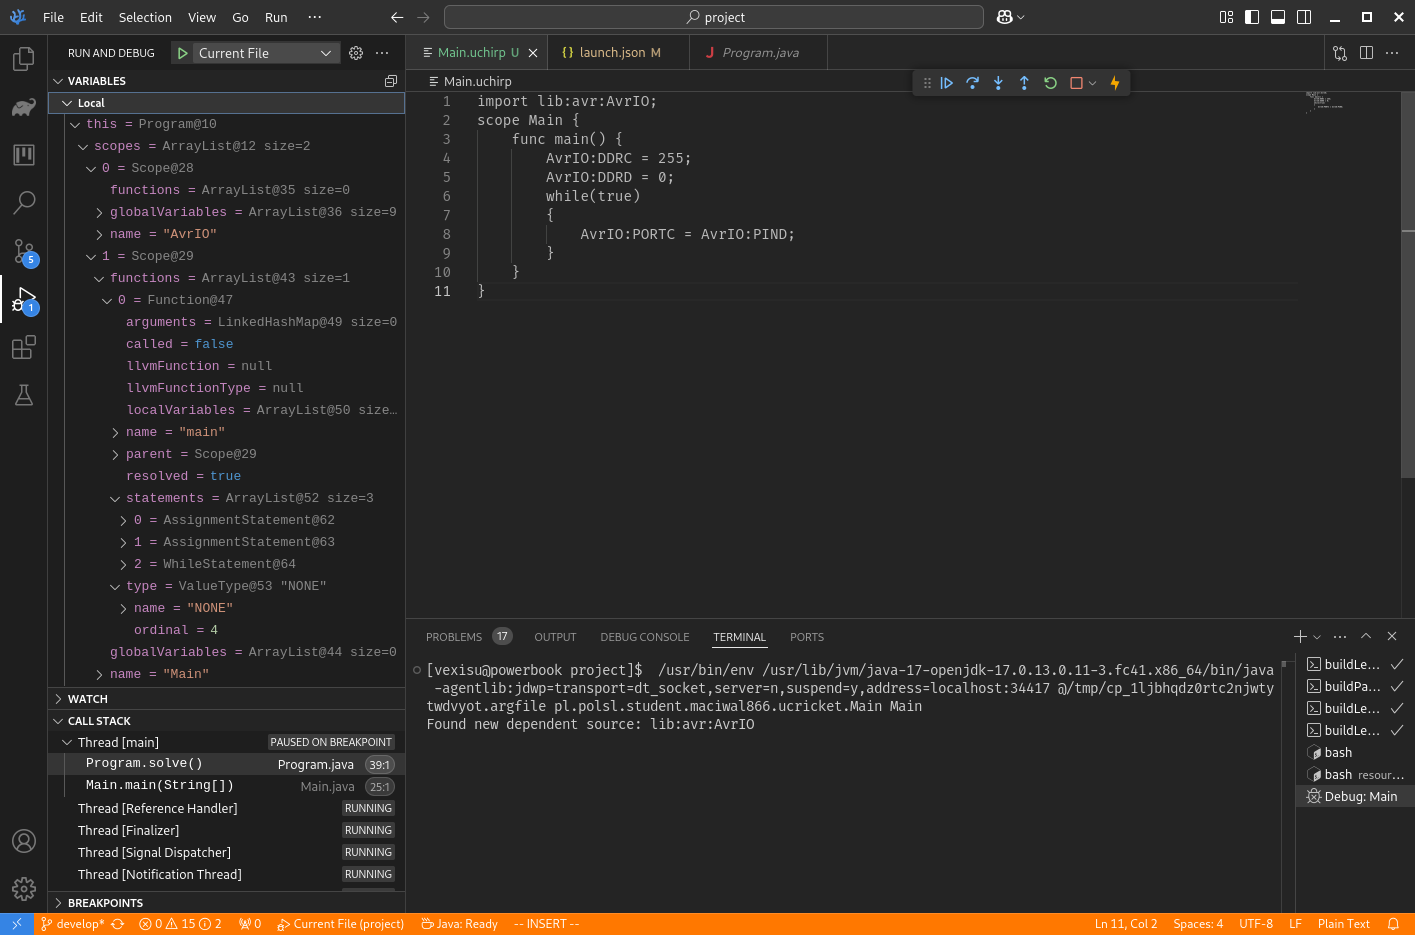
\includegraphics[width=1\textwidth]{graf/vscodium-debug-ast.png}
	\caption{Proces kontroli drzewa syntaktycznego za pomocą debugera wbudowanego w środowisko VSCodium.}
\label{fig:vscodium-debug-ast}
\end{figure}

\section{Poprawność generowanego kodu pośredniego}
Narzędzie LLVM posiada wbudowany system kontroli poprawności budowanej reprezentacji pośredniej. Odpowiada za to odpowiedna funkcje \lstinline|LLVMVerifyModule()| dostarczana przez API (ang. \english{application programming interface}), przedstawiona w kodzie źródłowym \ref{lst:ir-verify}. Wykorzystanie jej w połączeniu z funkcją \lstinline|LLVMDisposeMessage()| pozwala na weryfikację błędów w budowanej reprezentacji pośredniej. W szczególnych przypadkach, wymagane było krokowe przejście przez program narzędziem do debugowania, np. podczas przekazania nieodpowiedniej referencji typu zawartej w klasie \lstinline|LLVMTypeRef|, powodując tym samym błąd naruszenia ochrony pamięci.

\begin{lstlisting}[caption={Kod wywołujący kontrolę generowanej reprezentacji pośredniej.}, label={lst:ir-verify}]
var moduleMessage = new PointerPointer<BytePointer>(1);
LLVMVerifyModule(module, 0, moduleMessage);
LLVMDisposeMessage(moduleMessage.get(BytePointer.class)); 
\end{lstlisting}

Kolejnym mechanizmem pozwalającym na sprawdzenie poprawności kodu pośredniego było wygenerowanie jego reprezentacji w formie tekstowej przy użyciu funkcji \lstinline|LLVMDumpModule()|. Przekazuje ona na wyjście programu kompilatora odpowiednio sformatowaną reprezentację kodu pośredniego, którą można porównać z przygotowanym kodem testowym. Rysunek \ref{fig:ir-module-dump} przedstawia wygenerowaną reprezentację pośrednią wraz z testowanym kodem.

\begin{figure}
\centering
	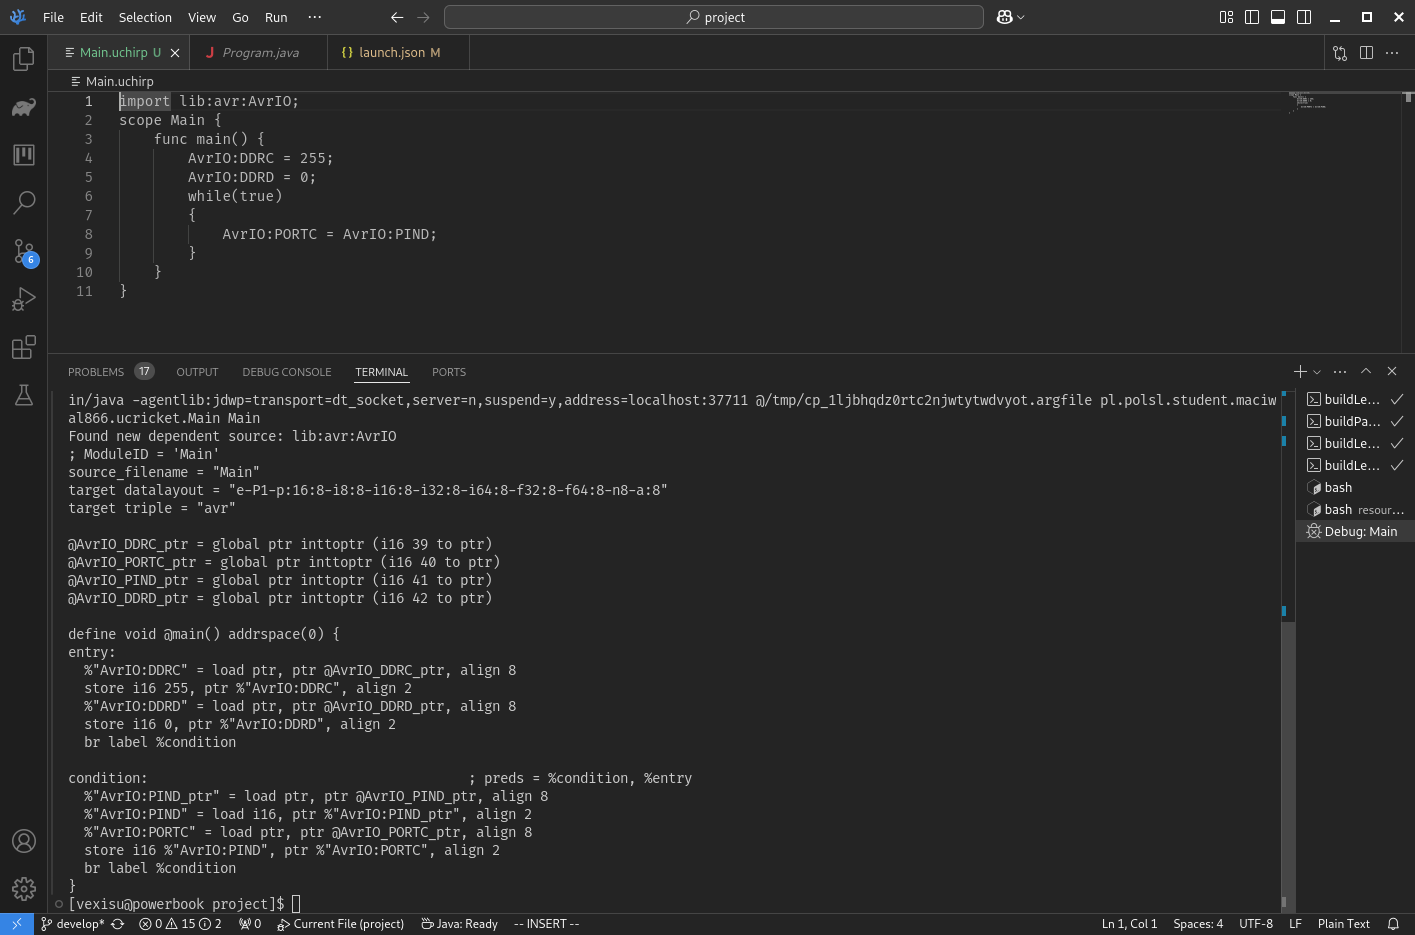
\includegraphics[width=1\textwidth]{graf/ir-module-dump.png}
	\caption{Testowy kod źródłowy wraz z jego reprezentacją pośrednią wygenerowaną przez LLVM.}
	\label{fig:ir-module-dump}
\end{figure}

\section{Poprawność kodu dla platformy wynikowej}
W trakcie generowania kodu wynikowego z poziomu narzędzia LLVM otrzymywany jest kod w języku Assembly. Jest to ostateczna czytelna forma programu dostępna dla użytkownika kompilatora. Na tym etapie kompilacji możliwe było sprawdzenie poprawności pogramu pod względem zarządzania pamięcią i wykonywanych instrukcji na procesorze mikrokontrolera. Kod języka Assembly jest dużo bardziej szczegółowy niż reprezentacja pośrednia dostarczana z narzędzia LLVM. Rysunek \ref{fig:compiled-asm-vs-ir} przedstawia finalny kod wygenerwoany przez LLVM wraz z jego reprezentacją pośrednią. 

\begin{figure}
	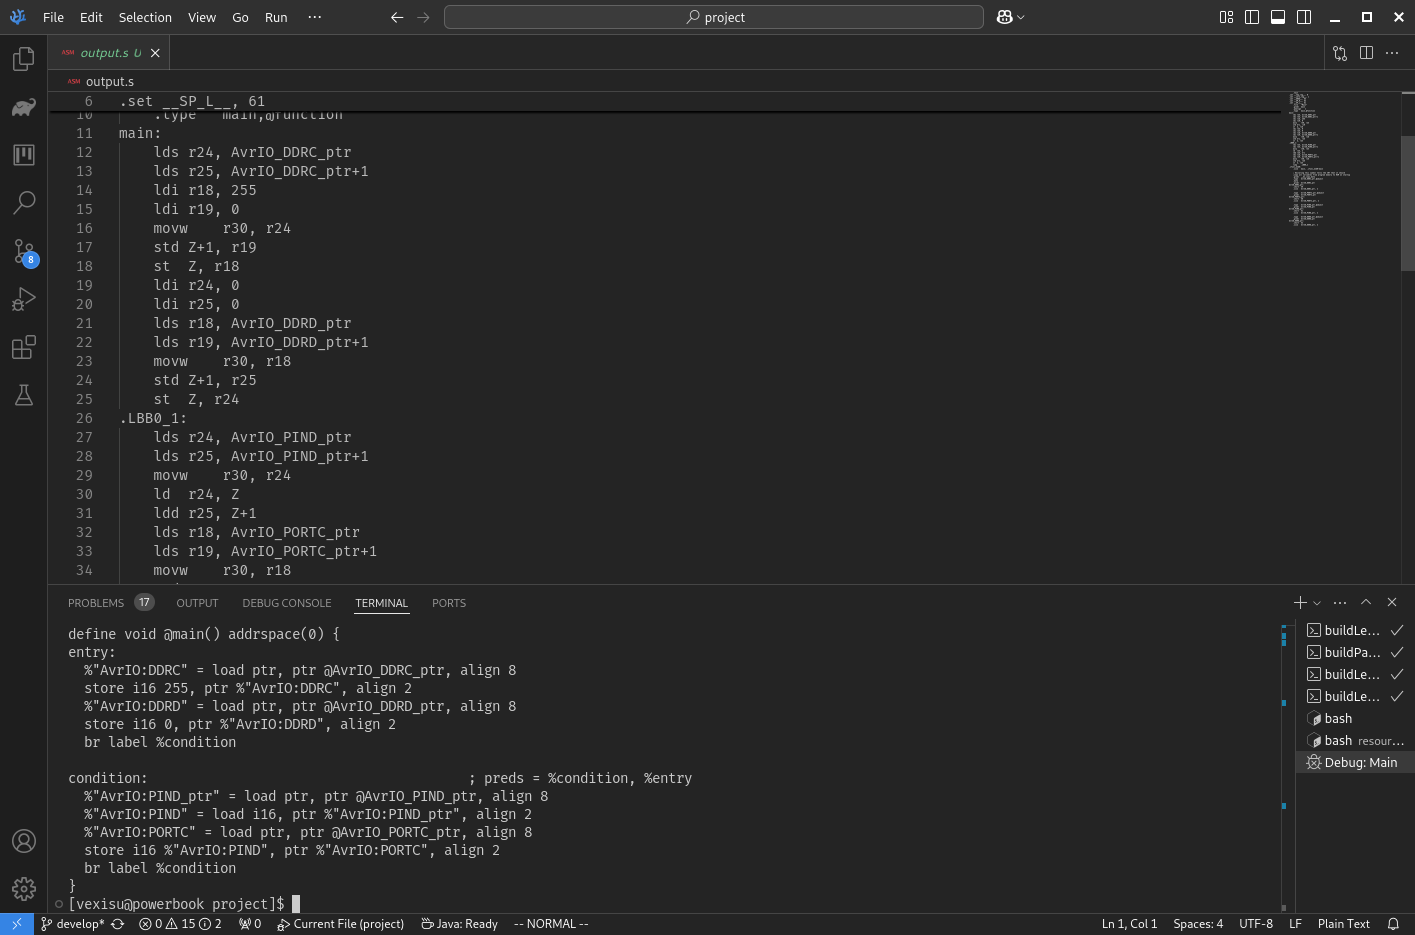
\includegraphics[width=1\textwidth]{graf/compiled-asm-vs-ir.png}
	\caption{Kod wynikowy w języku Assembly wraz z jego reprezentacją pośrednią.}
	\label{fig:compiled-asm-vs-ir}
\end{figure}

Kod binarny dla platformy docelowej uzyskany zostaje poprzez kompilację przy użyciu narzędzia avr-gcc. Testowanie pliku binarnego wymaga użycia odpowiedniego narzędzia pozwalającego na odczytanie instrukcji zakodowanych w formacie zrozumiałym dla mikrokontrolera. Do tego zadania użyto narzędzie Cutter. Jego głównym zastosowaniem jest inżyniera wsteczna kodu binarnego. Oferuje ono także debugowanie skompilowanych programów poprzez wbudowany symulator. Instrukcje programu prezentowane są wraz z odpowiednimi komentarzami akcji. Możliwe jest też przedstawienie kodu jako graf przepływu (rysunek \ref{fig:cutter-graph}). Dzięki niemu możliwa była krokowa analiza zachowania programu wraz z podglądem pamięci i rejestrów symulowanego mikrokontrolera. Rysunek \ref{fig:cutter-debug} prezentuje proces debugowania kodu wynikowego w programie Cutter. 

\begin{figure}
	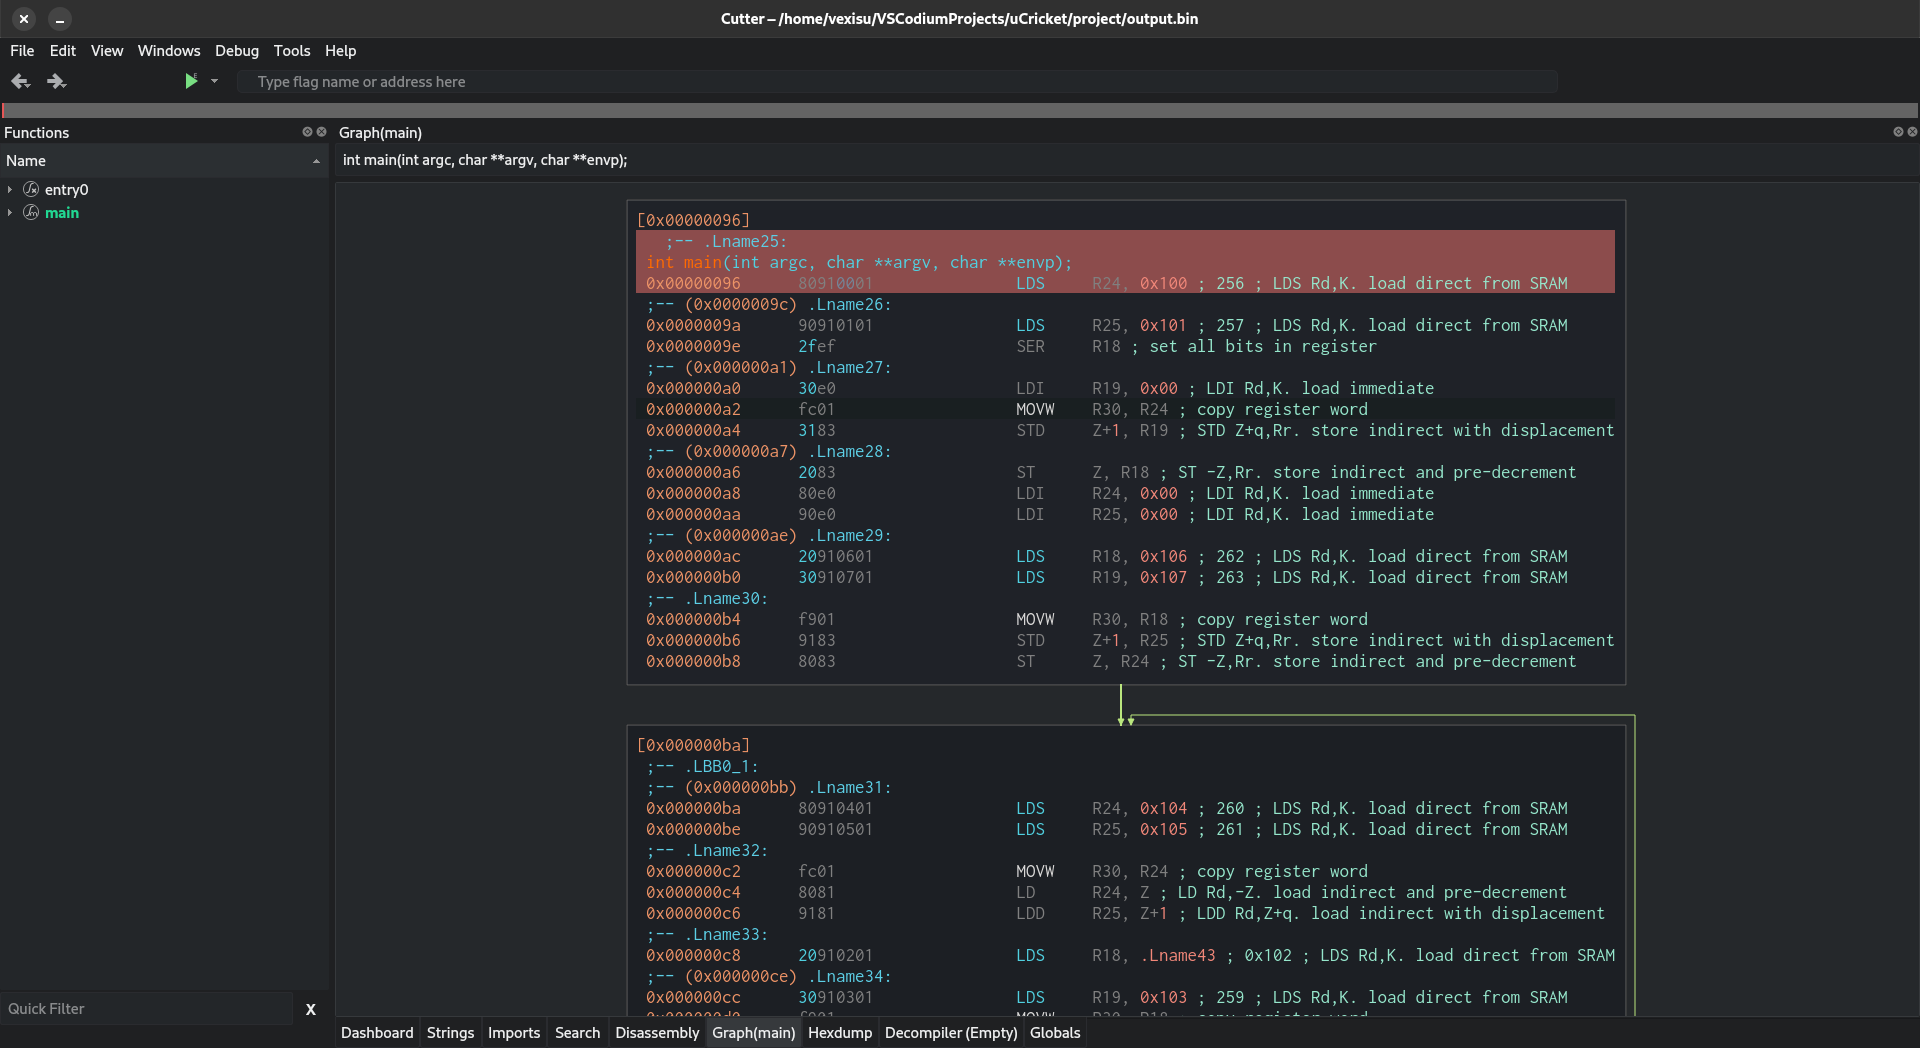
\includegraphics[width=1\textwidth]{graf/cutter-graph.png}
	\caption{Kod wynikowy w formie grafu prepływu prezentowanego w programie Cutter.}
	\label{fig:cutter-graph}
\end{figure}

\begin{figure}
	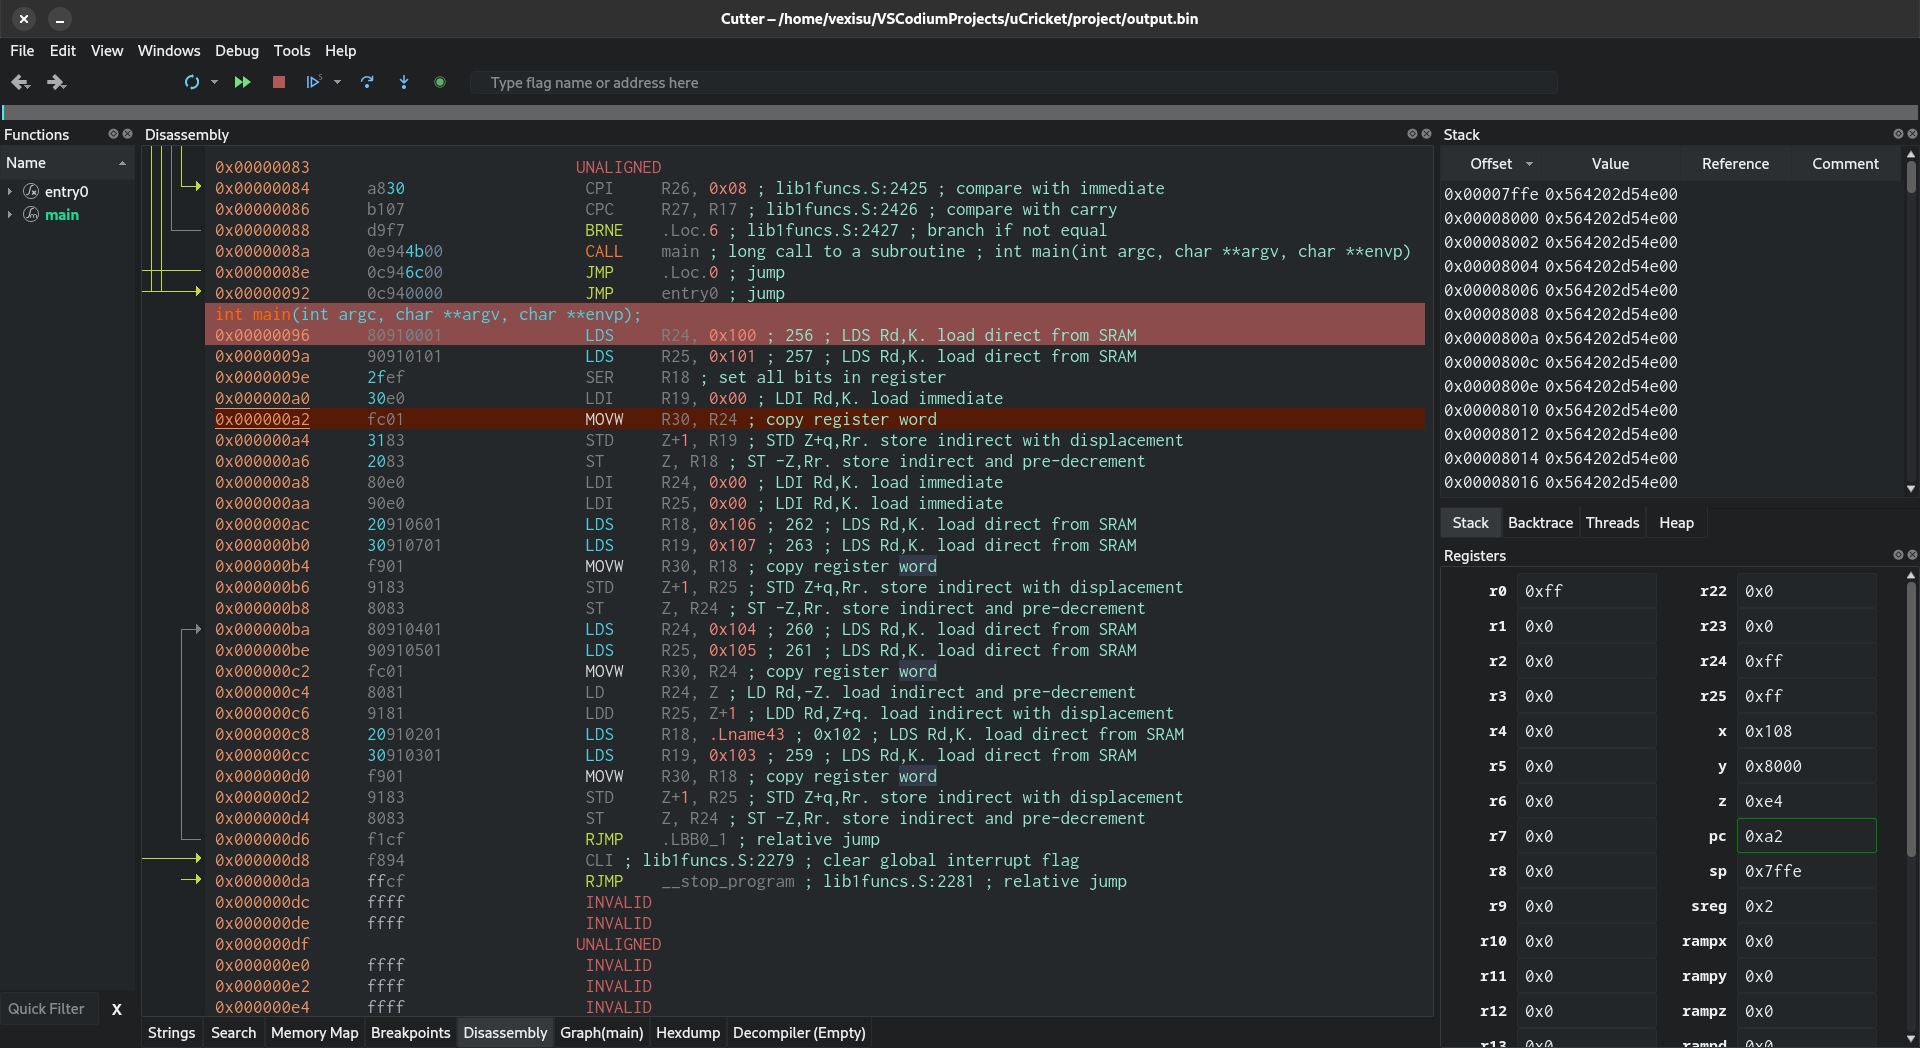
\includegraphics[width=1\textwidth]{graf/cutter-debug.png}
	\caption{Proces debugowania kodu wynikowego w programie Cutter.}
	\label{fig:cutter-debug}
\end{figure}

Program wynikowy został także przetestowany na platformie docelowej skłającej się z płytki rozwojowej Arduino Mini Pro posiadającej mikrokontroler ATmega328P. Prezentowany program wymagał także skonstruowanie układu z diod, przełączników i odpowiednich komponentów pasywnych. Rysunki \ref{fig:schematic} i \ref{fig:electronics} prezentują schemat i układ na którym testowano program. Programowanie mikrokontrolera odbyło się przy użyciu programatora USBasp.

\begin{figure}
	\textit{Tutaj zostanie dodany schemat}
	\caption{Schemat układu wykorzystanego do przetestowania programu.}
	\label{fig:schematic}
\end{figure}

\begin{figure}
	\textit{Tutaj zostanie dodane zdjęcie układu}
	\caption{Układ przeznaczony do testowania programu.}
	\label{fig:electronics}
\end{figure}

\begin{itemize}
\item sposób testowania w ramach pracy (np. odniesienie do modelu V)
\item organizacja eksperymentów
\item przypadki testowe zakres testowania (pełny/niepełny)
\item wykryte i usunięte błędy
\item opcjonalnie wyniki badań eksperymentalnych
\end{itemize}

%\begin{table}
%\centering
%\caption{Nagłówek tabeli jest nad tabelą.}
%\label{id:tab:wyniki}
%\begin{tabular}{rrrrrrrr}
%\toprule
%	         &                                     \multicolumn{7}{c}{metoda}                                      \\
%	         \cmidrule{2-8}
%	         &         &         &        \multicolumn{3}{c}{alg. 3}        & \multicolumn{2}{c}{alg. 4, $\gamma = 2$} \\
%	         \cmidrule(r){4-6}\cmidrule(r){7-8}
%	$\zeta$ &     alg. 1 &   alg. 2 & $\alpha= 1.5$ & $\alpha= 2$ & $\alpha= 3$ &   $\beta = 0.1$  &   $\beta = -0.1$ \\
%\midrule
%	       0 &  8.3250 & 1.45305 &       7.5791 &    14.8517 &    20.0028 & 1.16396 &                       1.1365 \\
%	       5 &  0.6111 & 2.27126 &       6.9952 &    13.8560 &    18.6064 & 1.18659 &                       1.1630 \\
%	      10 & 11.6126 & 2.69218 &       6.2520 &    12.5202 &    16.8278 & 1.23180 &                       1.2045 \\
%	      15 &  0.5665 & 2.95046 &       5.7753 &    11.4588 &    15.4837 & 1.25131 &                       1.2614 \\
%	      20 & 15.8728 & 3.07225 &       5.3071 &    10.3935 &    13.8738 & 1.25307 &                       1.2217 \\
%	      25 &  0.9791 & 3.19034 &       5.4575 &     9.9533 &    13.0721 & 1.27104 &                       1.2640 \\
%	      30 &  2.0228 & 3.27474 &       5.7461 &     9.7164 &    12.2637 & 1.33404 &                       1.3209 \\
%	      35 & 13.4210 & 3.36086 &       6.6735 &    10.0442 &    12.0270 & 1.35385 &                       1.3059 \\
%	      40 & 13.2226 & 3.36420 &       7.7248 &    10.4495 &    12.0379 & 1.34919 &                       1.2768 \\
%	      45 & 12.8445 & 3.47436 &       8.5539 &    10.8552 &    12.2773 & 1.42303 &                       1.4362 \\
%	      50 & 12.9245 & 3.58228 &       9.2702 &    11.2183 &    12.3990 & 1.40922 &                       1.3724 \\
%\bottomrule
%\end{tabular}
%\end{table}  
%
 % Weryfikacja i walidacja

% TODO
\chapter{Podsumowanie i wnioski}
\begin{itemize}
\item uzyskane wyniki w świetle postawionych celów i zdefiniowanych wyżej wymagań
\item kierunki ewentualnych danych prac (rozbudowa funkcjonalna …)
\item problemy napotkane w trakcie pracy
\end{itemize}

 % Podsumowanie i wnioski

\backmatter

%\bibliographystyle{plplain}  % bibtex
%\bibliography{biblio/biblio} % bibtex
\printbibliography           % biblatex
\addcontentsline{toc}{chapter}{Bibliografia}

\begin{appendices}

% TODO
\chapter{Spis skrótów i symboli}

\begin{itemize}
\item[LALR(1)] kwas deoksyrybonukleinowy (ang. \english{deoxyribonucleic acid})
\item[LLVM] model -- widok -- kontroler (ang. \english{model--view--controller}) 
\end{itemize}
 % Spis skrótów i symboli

% TODO
\chapter{Źródła}

Jeżeli w pracy konieczne jest umieszczenie długich fragmentów kodu źródłowego, należy je przenieść w to miejsce.

\begin{lstlisting}
if (_nClusters < 1)
	throw std::string ("unknown number of clusters");
if (_nIterations < 1 and _epsilon < 0)
	throw std::string ("You should set a maximal number of iteration or minimal difference -- epsilon.");
if (_nIterations > 0 and _epsilon > 0)
	throw std::string ("Both number of iterations and minimal epsilon set -- you should set either number of iterations or minimal epsilon.");
\end{lstlisting}


% % % % % % % % % % % % % % % % % % % % % % % % % % % % % % % % % % % 
% Pakiet minted wymaga odkomentowania w pliku config/settings.tex   %
% importu pakietu minted: \usepackage{minted}                       %
% i specjalnego kompilowania:                                       %
% pdflatex -shell-escape praca                                      %
% % % % % % % % % % % % % % % % % % % % % % % % % % % % % % % % % % % 

%\begin{minted}[linenos,breaklines,frame=lines]{c++}
%if (_nClusters < 1)
%   throw std::string ("unknown number of clusters");
%if (_nIterations < 1 and _epsilon < 0)
%   throw std::string ("You should set a maximal number of iteration or minimal difference -- epsilon.");
%if (_nIterations > 0 and _epsilon > 0)
%   throw std::string ("Both number of iterations and minimal epsilon set -- you should set either number of iterations or minimal epsilon.");
%\end{minted}
 % Źródła

% TODO
\chapter{Lista dodatkowych plików, uzupełniających tekst pracy} 


W systemie do pracy dołączono dodatkowe pliki zawierające:
\begin{itemize}
\item źródła programu,
\item dane testowe,
\item film pokazujący działanie opracowanego oprogramowania lub zaprojektowanego i~wykonanego urządzenia,
\item itp.
\end{itemize}
 % Lista dodatkowych plików, uzupełniających tekst pracy

\listoffigures
\addcontentsline{toc}{chapter}{Spis rysunków}
\listoftables
\addcontentsline{toc}{chapter}{Spis tabel}

\end{appendices}

\end{document}


%% Finis coronat opus.

